% DRL addresses sequential decision-making problems that can be formulated as Markov decision (MDP) processes~\cite{712192}. An MDP is defined by five elements: the state set ($S$), the action set ($A$), the state transition probability ($P$), the reward function ($R$), and the discount factor ($\gamma$). At each time step $t$, the agent observes the current state $s_t\!\in\!S$, selects an action $a_t\!\in\!A$ according to a policy $\pi$, and receives a reward $r_{t+1}$ while the environment transitions to a new state $s_{t+1}$, as illustrated in Fig.~\ref{fig:MDP}. Typically, the goal of an MDP problem is to achieve the maximum cumulative reward $R(t)$, which is:

% \begin{equation}
% R_t = r_{t} + \gamma r_{t+1} + \gamma^2 r_{t+2} + \cdots = \sum_{k=0}^{\infty} \gamma^{k} r_{t+k}
% \end{equation}

% The policy $\pi$ is characterized by two fundamental value functions: 
% the state-value function $V(s)$ and the action-value function $Q(s,a)$, 
% which represent the expected return from a state or from a specific state-action pair, respectively. 
% Their recursive definitions, referred to as the Bellman equations, are expressed as follows:  

% % --- State-value Bellman equation (compact IEEE-compliant) ---
% % \begin{align}
% % --- State-value Bellman equation (IEEE two-column compliant) ---
% \begin{align}
% V^\pi(s_t)
% &= \mathbb{E}\!\left[r_t + \gamma V^\pi(s_{t+1}) \mid s_t \right] \nonumber \\[-3pt]
% &= \sum_{a_t}\!\pi(a_t|s_t)
%    \sum_{s_{t+1},r_t}\!p(s_{t+1},r_t|s_t,a_t)
%    [\,r_t + \gamma V^\pi(s_{t+1})\,]
% \label{eq:state_value_function_st}
% \end{align}

% % --- Action-value Bellman equation (IEEE two-column compliant) ---
% \begin{align}
% Q^\pi(s_t,a_t)
% &= \mathbb{E}\!\left[r_t + \gamma Q^\pi(s_{t+1},a_{t+1})
%    \mid s_t,a_t \right] \nonumber \\[-3pt]
% &= \sum_{s_{t+1},r_t}\!p(s_{t+1},r_t|s_t,a_t)
%    \big[r_t + \gamma \!\sum_{a_{t+1}}\!
%    \pi(a_{t+1}|s_{t+1})  \nonumber \\[-3pt]
% &\quad\quad\quad\quad\quad\quad\quad\quad\quad\;\; \times Q^\pi(s_{t+1},a_{t+1})\big].
% \label{eq:action_value_function_st}
% \end{align}


% \noindent
% where \(p(s_{t+1},r_t|s_t,a_t)\) denotes the joint transition-reward probability describing the stochastic environment dynamics. 

% These formulations constitute the mathematical foundation for value estimation in DRL, underpinning most value-based and actor-critic algorithms employed in power electronic converter applications.Building upon this formulation, DRL algorithms aim to approximate the optimal policy that maximizes the expected return by learning from repeated interactions with the environment. Depending on how the environment model and policy optimization are realized, DRL techniques can be categorized as follows.

% \begin{figure}[!t]
%   \centering
%   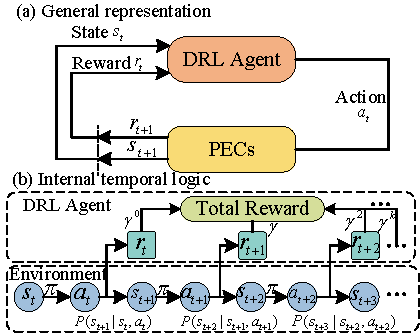
\includegraphics[width=\linewidth]{fig/MDP5.pdf}
%   \caption{The fundamentals of the MDP: (a) general representation and (b) internal temporal logic.}
%   \label{fig:MDP}
% \end{figure}

% \subsection{Algorithmic Taxonomy}
% \label{sec:taxonomy}

% DRL algorithms are broadly classified as model-based or model-free. 
% Model-based DRL employs an explicit environment model to predict future states and enhance sample efficiency; however, the nonlinear switching behavior of PECs makes accurate model construction challenging. 
% Consequently, most converter applications adopt model-free DRL, which learns policies directly from interaction data. 
% Model-free DRL can be further grouped by its action-selection mechanism into \emph{value-based}, \emph{policy-based}, and \emph{actor-critic (AC)}. 
% An additional paradigm, \emph{multi-agent DRL}, extends these foundations to systems with multiple cooperative or competitive agents. 
% Figure~\ref{fig:DRL_Task_Distribution2} summarizes the taxonomy of DRL algorithms and their life-cycle applications in PECs, and Table~\ref{tab:model_free_rl} outlines their principal characteristics.

% \begin{figure*}[!t]
%   \centering
%   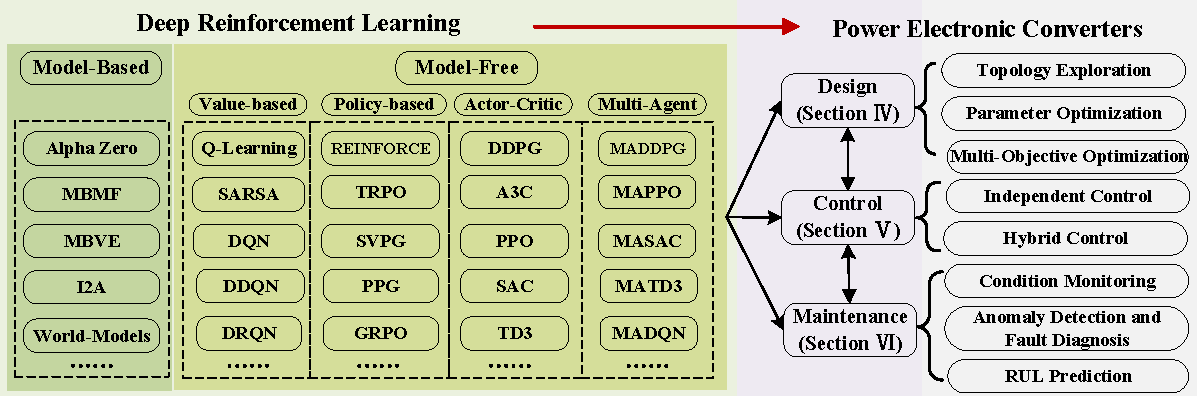
\includegraphics[width=0.8\textwidth]{fig/DRL_Task_Distribution6.pdf}
%   \caption{Taxonomy and life-cycle applications of DRL in PECs.}
%   \label{fig:DRL_Task_Distribution2}
% \end{figure*}

% \begin{table*}[!t]
% \centering
% \caption{Key Characteristics of Model-Free DRL Algorithm Families}
% \label{tab:model_free_rl}
% \begin{tabular}{lp{5cm}p{3.5cm}p{4.3cm}p{2cm}}
% \toprule
% \textbf{Category} & \textbf{Mechanism} & \textbf{Advantages} & \textbf{Disadvantages} & \textbf{Applicability} \\
% \midrule
% Value-based & Computes the value function and selects the action corresponding to the maximum value. & High sample efficiency, low estimation variance, reduced risk of local optima. & Less effective for continuous action problems, prone to overfitting, applicable mainly to low-dimensional problems. & Discrete \\
% \addlinespace
% \hline
% Policy-based & Directly selects actions that maximize cumulative returns without relying on the value function. & Effective for high-dimensional and continuous action spaces, better convergence properties. & High estimation variance, computationally expensive, low sample efficiency, susceptible to local optima. & Discrete \newline Continuous \\
% \addlinespace
% \hline
% Actor-Critic & The actor updates the policy based on the value function, while the critic estimates the value. & High sample utilization, reduced variance in value estimation, faster training. & Algorithm instability, sensitivity to hyperparameters. & Discrete \newline Continuous \\
% \addlinespace
% \hline
% Multi-agent & Multiple agents interact in a shared environment, learning cooperatively or competitively. & Models complex environments; enhances scalability and robustness; fosters cooperation or competition. & High complexity, non-stationary environment for each agent, communication and computation overhead, convergence issues. & Discrete \newline Continuous \\
% \bottomrule
% \end{tabular}
% \end{table*}

% \subsection{Value-Based Methods}
% \label{sec:value_methods}

% Among the model-free DRL families, value-based algorithms represent the most fundamental class and have been extensively investigated for converter optimization and control. 
% These methods estimate the expected return associated with each state or state-action pair and derive an optimal policy by maximizing the corresponding value function. 
% Representative algorithms include state-action-reward-state-action (SARSA)~\cite{rummery1994line}, Q-learning (QL)~\cite{watkins1992q}, deep Q-network (DQN)~\cite{van2016deep}, and double DQN (DDQN)~\cite{wang2016dueling}. 
% SARSA updates its Q-table under an exploratory policy, thereby maintaining continuous exploration of the state-action space, whereas QL employs a greedy strategy that accelerates exploitation of the learned value function. 
% Both algorithms converge efficiently in discrete environments but are restricted by the finite nature of their state representations. 
% The DQN extends these methods by replacing tabular Q-values with neural-network approximations, enabling learning in continuous and high-dimensional state spaces. 
% The DDQN further mitigates the overestimation tendency of DQN by decoupling the processes of action selection and value evaluation. 
% In converter control, value-based DRL has demonstrated particular effectiveness in switched or quantized control applications, such as discrete duty-cycle regulation and operation-mode selection.

% In summary, value-based DRL methods offer high sample efficiency, low variance in value estimation, and notable robustness against local optima. 
% Nevertheless, their performance remains constrained by discrete or low-dimensional action spaces and is often susceptible to overfitting when extended to continuous domains. 
% Despite these limitations, value-based approaches constitute the algorithmic foundation of DRL, forming essential components of hybrid and actor-critic architectures widely employed in converter control.To overcome these limitations, policy-based algorithms have been developed, which directly optimize the control policy without relying on explicit value estimation. 
% This paradigm shift enables continuous and smooth control, making policy-based DRL particularly suitable for converter applications requiring fine-grained modulation or adaptive regulation.

% \subsection{Policy-Based Methods}
% \label{sec:policy_methods}
% % proximal policy optimization (PPO)~\cite{schulman2017proximal}

% Policy-based algorithms directly optimize the policy parameters to maximize the objective function without explicit value estimation. 
% Representative methods include REINFORCE~\cite{williams1992simple}, trust-region policy optimization (TRPO)~\cite{schulman2015trust}, Stein variational policy gradient (SVPG)~\cite{liu2017stein}, and generalized regularized policy optimization (GRPO)~\cite{shao2024deepseekmath}. 
% The REINFORCE algorithm, introduced by Williams in 1992, represents the earliest formulation of stochastic policy-gradient optimization, providing a foundation for subsequent policy-search frameworks.  
% Despite its conceptual simplicity, REINFORCE relies on Monte Carlo (MC) returns, resulting in high gradient variance and slow convergence. 
% TRPO advanced this approach by constraining the policy update step within a trust region, ensuring monotonic improvement and enhanced stability.  
% SVPG introduces a probabilistic variational formulation to enhance exploration, whereas GRPO regularizes the policy gradient to improve generalization and prevent overfitting.  
% In converter systems, policy-based DRL is particularly advantageous for continuous-action control, such as duty-ratio modulation or phase-shift regulation, where smooth action generation is required.

% In summary, policy-based DRL methods offer strong convergence properties and handle continuous action spaces effectively. 
% However, they often suffer from high variance in gradient estimation, low sample efficiency, and instability in training. 
% To address these challenges, actor-critic algorithms were developed to integrate value-based evaluation with policy optimization, combining the strengths of both paradigms for improved stability and learning efficiency.

% \subsection{Actor-Critic Methods}
% \label{sec:ac_methods}

% Actor-critic (AC) algorithms integrate the strengths of value- and policy-based approaches through two coupled networks: the actor (policy) and the critic (value). 
% Representative variants include deep deterministic policy gradient (DDPG)~\cite{lillicrap2015continuous}, asynchronous advantage actor-critic (A3C)~\cite{mnih2016asynchronous}, Proximal Policy Optimization (PPO)~\cite{schulman2017proximal}, twin-delayed DDPG (TD3)~\cite{fujimoto2018addressing}, and soft actor-critic (SAC)~\cite{haarnoja2018soft}. 
% Although PPO originated from the policy-gradient family, it is widely recognized as a policy-gradient-based actor–critic algorithm because it jointly optimizes a clipped surrogate objective with a value-function baseline to stabilize updates and reduce policy oscillation.
% DDPG extends the AC framework to continuous action spaces but tends to overestimate Q-values, whereas TD3 mitigates this issue through dual critics and delayed policy updates. 
% A3C enhances sample efficiency via parallel asynchronous training, while SAC introduces entropy regularization to improve exploration and ensure stable convergence.  
% In converter applications, AC algorithms have demonstrated robust performance in nonlinear and high-dimensional control problems, achieving fast convergence while maintaining resilience to modeling uncertainties.

% In summary, AC algorithms inherit the strengths of both value-based and policy-based methods, offering lower variance in value estimation, higher sample efficiency, and faster overall convergence. 
% Nevertheless, their performance remains sensitive to hyperparameter tuning and network configuration, and their computational complexity increases with system dimensionality.

% \subsection{Multi-Agent Methods}
% \label{sec:multi_agent_methods}

% Extending beyond single-agent paradigms, multi-agent DRL generalizes value-based, policy-based, and actor–critic-based frameworks into decentralized systems, where multiple agents learn concurrently through cooperation or competition. The underlying mathematical model transitions from a MDP to a Markov game (MG), in which the reward of each agent depends on joint actions and shared environmental dynamics.
% Representative algorithms include multi-agent DDPG (MADDPG)~\cite{lowe2017multi}, multi-agent PPO (MAPPO)~\cite{yu2022surprising}, multi-agent TD3 (MATD3)~\cite{ackermann2019reducing}, and multi-agent SAC (MASAC)~\cite{kuba2021trust}. 
% These frameworks often adopt centralized critics, shared policies, or entropy regularization to improve coordination, scalability, and robustness in multi-agent environments.  
% In converter networks—such as modular multilevel converters, distributed inverters, and microgrid clusters—MARL facilitates cooperative power sharing, fault-tolerant operation, and adaptive energy management among converter modules, providing a scalable foundation for distributed intelligent control in future power-electronic systems.

% In summary, multi-agent DRL provides a scalable extension of single-agent frameworks, enabling cooperative and competitive behaviors across distributed converter systems. 
% By leveraging shared critics and communication mechanisms, these algorithms enhance coordination and robustness in complex, interconnected environments. 
% However, their deployment remains computationally intensive and sensitive to communication delays or partial observability, motivating further research on lightweight and communication-efficient architectures. 

% The following subsection summarizes these algorithmic families and discusses their overall relevance to power-electronic converter applications.

% \subsection{Summary and Relevance to PECs}
% \label{sec:drl_summary}

% Across these algorithmic families, model-free DRL provides an adaptive and data-driven paradigm that mitigates dependence on precise converter models. 
% Through continual interaction with the operating environment, DRL agents can track time-varying parameters and sustain near-optimal performance under dynamic conditions. 
% By integrating perception, decision-making, and control within a unified learning architecture, DRL effectively bridges the gap between model-based optimization and real-time adaptability in converter systems. 
% Consequently, it serves as a unifying methodology for topology design, control, and maintenance, forming the foundation for the next generation of intelligent, self-configurable power electronic converters. 

% Building on this foundation, the following section investigates the temporal evolution, utilization patterns, and emerging trends of DRL algorithms in PECs.

DRL addresses sequential decision-making problems that can be formulated as Markov decision (MDP) processes~\cite{712192}. 
An MDP is defined by five elements: the state set ($S$), the action set ($A$), the state-transition probability ($P$), the reward function ($R$), and the discount factor ($\gamma$). 
At each time step $t$, an agent observes the current state $s_t \in S$, selects an action $a_t \in A$ according to a policy $\pi$, and receives a reward $r_{t+1}$ as the environment transitions to a new state $s_{t+1}$, as illustrated in Fig.~\ref{fig:MDP}. 
The objective is to maximize the cumulative discounted reward $R_t$, defined as
\begin{equation}
R_t = \sum_{k=0}^{\infty} \gamma^{k} r_{t+k}
\end{equation}

The policy $\pi$ is characterized by two value functions: the state-value function $V(s)$ and the action-value function $Q(s,a)$, representing the expected return from a given state or state–action pair, respectively. 
Their recursive forms, known as the Bellman equations, are expressed as

\begin{align}
V^\pi(s_t)
&= \mathbb{E}\!\left[r_t + \gamma V^\pi(s_{t+1}) \mid s_t \right] \nonumber \\[-3pt]
&= \sum_{a_t}\!\pi(a_t|s_t)
   \sum_{s_{t+1},r_t}\!p(s_{t+1},r_t|s_t,a_t)
   [r_t + \gamma V^\pi(s_{t+1})]
\label{eq:state_value_function_st}
\end{align}

\begin{align}
Q^\pi(s_t,a_t)
&= \mathbb{E}\!\left[r_t + \gamma Q^\pi(s_{t+1},a_{t+1}) \mid s_t,a_t \right] \nonumber \\[-3pt]
&= \sum_{s_{t+1},r_t}\!p(s_{t+1},r_t|s_t,a_t)
   \big[r_t + \gamma \!\sum_{a_{t+1}}\!
   \pi(a_{t+1}|s_{t+1})  \nonumber \\[-3pt]
&\quad\quad\quad\quad\quad\quad\quad\quad Q^\pi(s_{t+1},a_{t+1})\big]
\label{eq:action_value_function_st}
\end{align}

\noindent
where \(p(s_{t+1},r_t|s_t,a_t)\) denotes the joint transition–reward probability describing the stochastic environment dynamics. 
These equations form the mathematical foundation for value estimation in DRL. 
They underpin most value-based and actor–critic algorithms that are employed in PEC applications. 
Building upon this foundation, DRL algorithms seek to approximate the optimal policy that maximizes the expected return through repeated interaction with the environment. 
Depending on how the environment model and policy optimization are realized, DRL techniques can be categorized as follows.

\begin{figure}[!t]
  \centering
  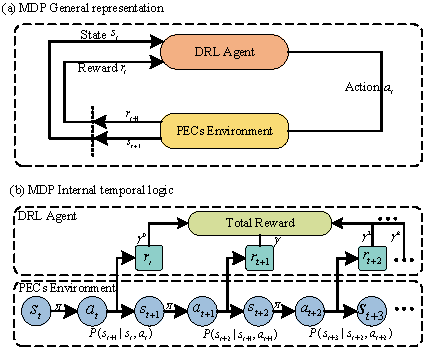
\includegraphics[width=\linewidth]{fig/MDP6.pdf}
  \caption{Fundamentals of the Markov decision process: (a) general representation and (b) internal temporal logic.}
  \label{fig:MDP}
\end{figure}

\subsection{Algorithmic Taxonomy}
\label{sec:taxonomy}

DRL algorithms are broadly classified as model-based or model-free. 
Model-based DRL employs an explicit model of the environment to predict future states and improve sample efficiency; however, the nonlinear switching behavior of PECs makes accurate model construction particularly difficult. 
Consequently, most converter applications adopt model-free DRL, which learns policies directly from data obtained through interaction. 
Model-free DRL algorithms can be further divided by their action-selection mechanism into \textit{value-based}, \textit{policy-based}, and \textit{actor–critic (AC)} methods. 
An additional paradigm, \textit{multi-agent DRL}, extends these principles to multi-agent systems in which several agents interact cooperatively or competitively. 
Figure~\ref{fig:DRL_Task_Distribution2} summarizes the taxonomy of DRL algorithms and their life-cycle applications in PECs, and Table~\ref{tab:model_free_rl} outlines their key characteristics.

\begin{figure*}[!t]
  \centering
  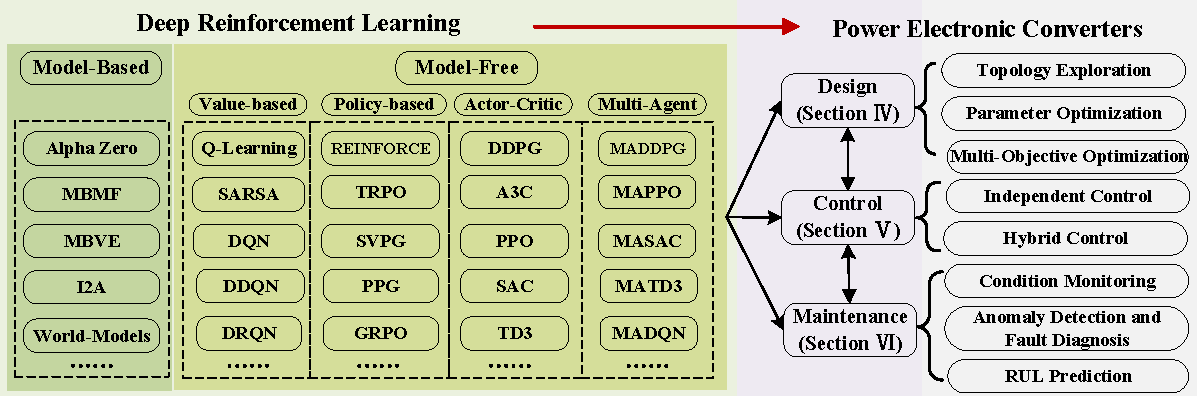
\includegraphics[width=0.8\textwidth]{fig/DRL_Task_Distribution6.pdf}
  \caption{Taxonomy and life-cycle applications of DRL in PECs.}
  \label{fig:DRL_Task_Distribution2}
\end{figure*}

\begin{table*}[t]
\centering
\caption{Condensed Characteristics of Model-Free DRL Algorithm Families}
\label{tab:model_free_rl}
\renewcommand{\arraystretch}{1.25}
\resizebox{\textwidth}{!}{
\begin{tabular}{@{}l l p{4.2cm} l p{5.2cm}@{}}
\toprule
\textbf{Category} & \textbf{Representative Algorithms} & \textbf{Mechanism} & \textbf{Applicability} & \textbf{Advantages (+) and Limitations (–)} \\ 
\midrule

Value-based & DQN / Double DQN &
Q-function approximation with \newline greedy action selection &
Discrete &
+ High sample efficiency \newline
+ Low estimation variance \newline
– Unsuitable for continuous control \newline
– Overestimation; limited scalability \\ 
\midrule

Policy-based & REINFORCE / TRPO / SVPG &
Direct policy optimization using \newline likelihood-ratio &
Discrete / Continuous &
+ High-dimensional action support \newline
+ Smooth/stable policy updates \newline
– High gradient variance \newline
– Low sample efficiency \\ 
\midrule

Actor–Critic & PPO / A3C / DDPG / SAC &
Coupled actor–critic learning with \newline bootstrapped value targets &
Discrete / Continuous &
+ Variance reduction \newline
+ Improved sample utilization \newline
– Hyperparameter sensitivity \newline
– Increased computational load \\ 
\midrule

Multi-agent & MADDPG / MAPPO / MASAC &
Decentralized/centralized training \newline for cooperative/competitive agents &
Discrete / Continuous &
+ Scalable coordination \newline
+ Robust emergent behaviors \newline
– Non-stationary environments \newline
– Credit assignment \\ 
\bottomrule
\end{tabular}}
\end{table*}




\subsection{Value-Based Methods}
\label{sec:value_methods}

Among model-free DRL families, value-based algorithms represent the earliest and most fundamental class. 
They estimate the expected return for each state–action pair and derive an optimal policy by maximizing the corresponding value function. 
Representative methods include state–action–reward–state–action (SARSA)~\cite{rummery1994line}, Q-learning (QL)~\cite{watkins1992q}, deep Q-network (DQN)~\cite{van2016deep}, and double DQN (DDQN)~\cite{wang2016dueling}. 
SARSA updates its Q-table using an exploratory policy to ensure continuous coverage of the state–action space, whereas QL employs a greedy strategy that accelerates exploitation of learned values. 
Both algorithms converge efficiently in discrete environments but are limited by finite state representations. 
DQN extends these methods by replacing tabular Q-values with neural network approximations, enabling learning in high-dimensional state spaces. 
DDQN further mitigates Q-value overestimation by decoupling action selection and value evaluation. 
In converter control, value-based DRL has proven effective for discrete switching tasks such as duty-cycle selection and mode transition management.

In summary, value-based methods offer high sample efficiency and low estimation variance, yet their reliance on discrete actions constrains scalability in continuous domains. 
They remain, however, the conceptual foundation of DRL, forming essential components of hybrid and actor–critic frameworks frequently employed in converter systems. 
To overcome their limitations, policy-gradient (PG) algorithms were subsequently developed to directly optimize control policies without explicit value estimation.

\subsection{Policy-Based Methods}
\label{sec:policy_methods}

Policy-based algorithms optimize the policy parameters to maximize the objective function directly. 
Representative methods include REINFORCE~\cite{williams1992simple}, trust-region policy optimization (TRPO)~\cite{schulman2015trust}, Stein variational policy gradient (SVPG)~\cite{liu2017stein}, and generalized regularized policy optimization (GRPO)~\cite{shao2024deepseekmath}. 
REINFORCE, introduced in 1992, provides the earliest formulation of stochastic policy-gradient optimization and establishes the foundation for subsequent research. 
Although conceptually straightforward, it depends on Monte Carlo returns, leading to high gradient variance and slow convergence. 
TRPO improves stability by constraining policy updates within a trust region, ensuring monotonic performance improvement. 
SVPG introduces a probabilistic variational framework that enhances exploration, while GRPO regularizes policy gradients to improve generalization and reduce overfitting. 
Within PECs, policy-based DRL is advantageous for continuous-action control, such as duty-ratio modulation and phase-shift regulation, where smooth and differentiable policy outputs are required.

In summary, policy-gradient methods effectively handle continuous action spaces and provide strong convergence guarantees, though they often exhibit high variance and low sample efficiency. 
To address these challenges, actor–critic algorithms integrate value estimation with policy optimization, combining the strengths of both paradigms.

\subsection{Actor–Critic Methods}
\label{sec:ac_methods}

Actor–critic (AC) algorithms combine policy-based and value-based learning through two coupled networks: the actor, which determines actions, and the critic, which evaluates them. 
Representative variants include deep deterministic policy gradient (DDPG)~\cite{lillicrap2015continuous}, asynchronous advantage actor–critic (A3C)~\cite{mnih2016asynchronous}, proximal policy optimization (PPO)~\cite{schulman2017proximal}, twin-delayed DDPG (TD3)~\cite{fujimoto2018addressing}, and soft actor–critic (SAC)~\cite{haarnoja2018soft}. 
Although PPO originated within the policy-gradient family, it is widely regarded as an actor–critic algorithm because it combines a clipped surrogate objective with a value-function baseline to stabilize learning and reduce policy oscillation. 
DDPG enables continuous deterministic control but tends to overestimate Q-values, a limitation addressed by TD3 through the use of twin critics and delayed target updates. 
A3C enhances sample efficiency by employing asynchronous parallel training, whereas SAC incorporates entropy regularization to improve exploration and convergence stability. 
In converter control, AC algorithms have demonstrated superior robustness in nonlinear, high-dimensional, and time-varying systems, achieving faster convergence and higher adaptability than purely value- or policy-based approaches.

In summary, AC algorithms inherit the advantages of both value and policy learning, providing high sample utilization and low variance in value estimation. 
Their performance, however, remains sensitive to hyperparameter configuration and network scaling, particularly in complex converter environments.

\subsection{Multi-Agent Methods}
\label{sec:multi_agent_methods}

Extending beyond single-agent paradigms, multi-agent DRL generalizes value-based, policy-based, and actor–critic frameworks into decentralized systems where multiple agents learn concurrently through cooperation or competition. 
The underlying mathematical formulation transitions from an MDP to a Markov game (MG), where each agent’s reward depends on the joint actions and shared environment dynamics. 
Representative methods include multi-agent DDPG (MADDPG)~\cite{lowe2017multi}, multi-agent PPO (MAPPO)~\cite{yu2022surprising}, multi-agent TD3 (MATD3)~\cite{ackermann2019reducing}, and multi-agent SAC (MASAC)~\cite{kuba2021trust}. 
These frameworks often employ centralized critics, shared policies, or entropy regularization to enhance coordination, scalability, and robustness. 
In converter networks such as modular multilevel converters, distributed inverters, and microgrid clusters, multi-agent reinforcement learning enables cooperative power sharing, fault-tolerant operation, and adaptive energy management, forming the foundation for distributed intelligent control.

In summary, multi-agent DRL extends single-agent frameworks to distributed systems, enabling cooperative and competitive learning across multiple converter modules. 
Although computationally demanding and sensitive to communication latency, these algorithms represent a promising direction for scalable, fault-tolerant converter coordination.

\subsection{Summary and Relevance to PECs}
\label{sec:drl_summary}

Across these algorithmic families, model-free DRL provides an adaptive and data-driven paradigm that mitigates dependence on precise converter models. 
By continuously interacting with the environment, DRL agents can adapt to time-varying parameters and sustain near-optimal performance under nonlinear operating conditions. 
Through the integration of perception, decision-making, and control within a unified learning architecture, DRL bridges the gap between model-based optimization and real-time adaptability in converter systems. 
While this section has outlined the theoretical taxonomy and algorithmic mechanisms of DRL, the following section transitions to a temporal perspective, examining how representative algorithms have evolved, diversified, and been adopted in PEC research over time.
\begin{figure*}[!t]
  \centering
  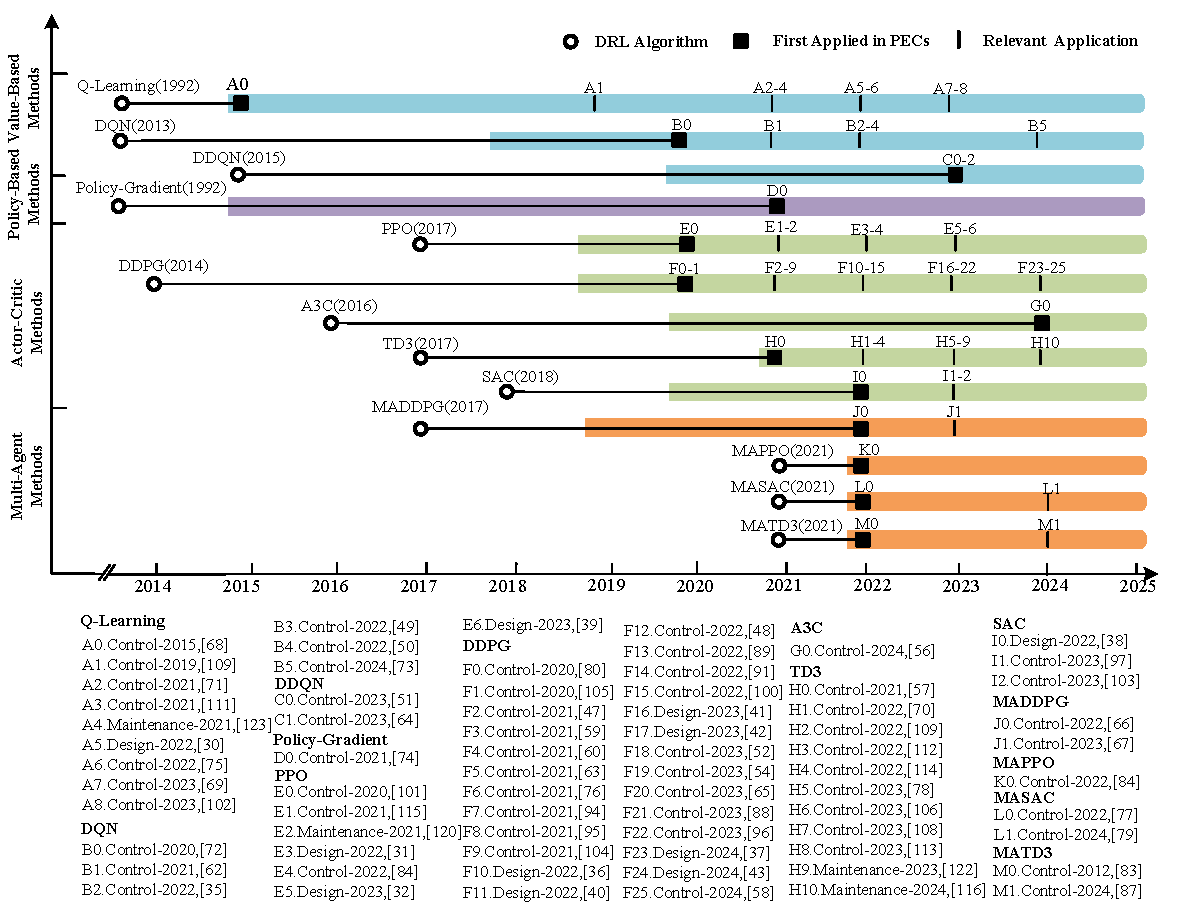
\includegraphics[width=0.9\textwidth]{fig/TIME_LINE7.pdf}
  \caption{Chronological evolution of representative DRL algorithms and their reported adoption in PECs applications.}
  \label{fig:DRL_Timeline}
\end{figure*}
